\setchapterimage[7cm]{ztf/ztf_telescope.png}
\chapter{The Nuclear Sample}\label{ztf}
\labch{nucsam}
Motivated by the three neutrinos coincident with accretion phenomena in the cores of active galaxies, it will be instructive to create a systematic sample of nuclear transients in the ZTF footprint. Furthermore, with the advent of a deep high-cadence sky survey like LSST in the near future\todo{source?}, photometric identification of transients will be crucial. The data volume created by LSST will by far exhaust the available spectroscopic resources, thus requiring informed decisions about when to apply spectroscopy. Classifying the ZTF nuclear transients is thus an important precursor study to LSST-era astronomy,

This chapter is dedicate to the nuclear sample, and is structured as follows: A discussion on the sample creation will be followed by different methods to classify the sample. This will be done with a special focus on TDEs.

\section{Sample Creation}
The nuclear sample was created with \texttt{AMPEL} (see Section~\ref{ampel}), using its capability to rerun analyses on archival data. To perform such a rerun, a modified version of the \texttt{AMPEL} nuclear filter was used.

\subsection{\texttt{AMPEL} Nuclear Filter}
The filter is used primarily by the ZTF TDE working group to scan for transient activity that is compatible with an emerging TDE~\cite{Velzen2021a}. In the rerun, it was slightly modified, and used to evaluate each and every alert issued by ZTF according to the following criteria:
\begin{description}
    \item[\texttt{sgscore}] As detailed in Section~\ref{ztf_image_subtraction}, \texttt{sgscore} is a machine-learning based star-galaxy score for PS1 objects (low values: galaxy, high values: stars). The transient must at least once have an \texttt{sgsscore} < 0.3 to pass the filter.
    \item[Number of detections] At least 3 detections across all bands are required.
    \item[Galactic cut] The object must be separated by at least \SI{5}{\degree} from the galactic plane.
    \item[PS1 photometry] To avoid crowded areas, transients where more than 100 objects in the vicinity have a counterpart in PS1 are removed.
    \item[Brightness] At least one alert datapoint of the transient must be brighter than 20 mag.
    \item[\texttt{rbscore}] The real-bogus score separating erroneous detections (low values) from real ones (high values, see Section~\ref{ztf_alerts}) must be larger than 0.3. Note that for more recent data, also \texttt{deep real bogus} is available, which promises vastly better results \sidecite{Duev2019}. Older alerts from 2018 or 2019 do not contain this information, and there is no direct translation from an \texttt{rbscore} threshold to a \texttt{drbscore} threshold. For these reasons and to maximize consistency, we restricted ourselves to using only the older \texttt{rbscore}. The quite loose cut of 0.3 does not entail overly large contamination, as we also require the transient to have a PS1 counterpart.
\end{description}

\begin{figure}[htpb]
    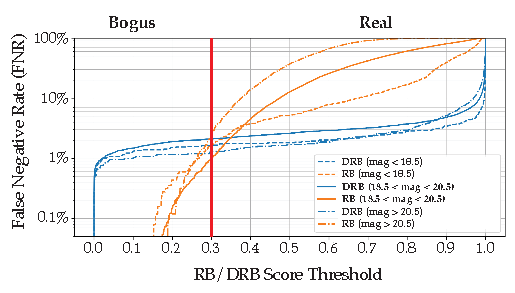
\includegraphics[width=0.9\textwidth]{nuclear/rb_v_drb.pdf}
    \caption[\texttt{rbscore}/\texttt{drbscore} performance]{\texttt{rbscore} vs \texttt{drbscore} performance, evaluated in terms of false negative rate as a function of the threshold. Adapted from~\cite{Duev2019}. The chosen threshold of 0.3 is shown as red vertical line. At that value, \texttt{rbscore} has a false negative rate of \SI{\approx 1}{\percent} in the relevant magnitude range of $18.5 < \text{mag} < 20.5$.}
    \labfig{rbvsdrb}
\end{figure}